\section{Practical Advantages of Open Source}\frame{\sectionpage}

\begin{frame}{Software for Freedom vs. Freedom for Software}
  \begin{column}{0.6\textwidth}
    \begin{itemize}
      \item Needs fulfilled by free software
        \begin{itemize}
          \item a need for software
          \item a need for ethical software and practices
        \end{itemize}
      \item Stallman's emphasis on a ``free digital society''
      \item Consequentialist stance on free software
        \begin{itemize}
          \item open source vs.\ free software
          \item a less radical approach
          \item weighing the utility of open source
          \item need-driven software~\cite[p. 17]{bisson}
        \end{itemize}
    \end{itemize}
  \end{column}
  \begin{column}{0.4\textwidth}\raggedleft
    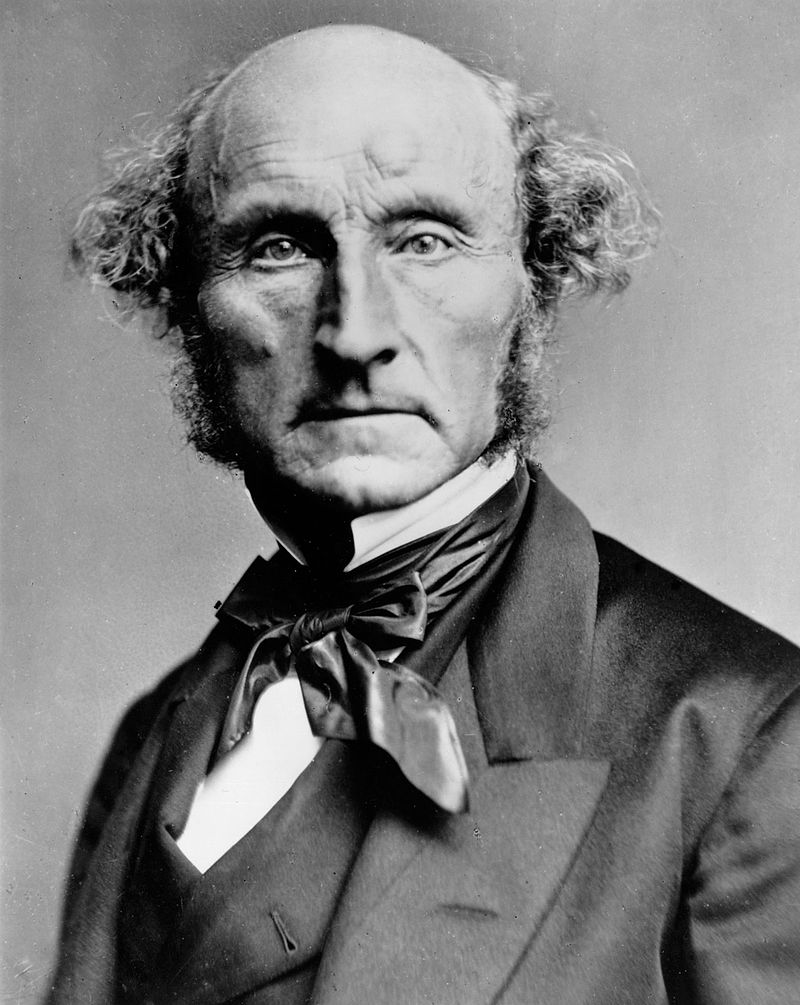
\includegraphics[width = 0.75\textwidth]{mill.jpg}
  \end{column}
\end{frame}

%%% include a citation for mill.jpg from https://en.wikipedia.org/wiki/John_Stuart_Mill


\begin{frame}{GNU + Linux, GNU/Linux}
  \begin{column}{0.5\textwidth}
    \begin{itemize}
      \item The GNU operating system
        \begin{itemize}
          \item ``written for your freedom''~\cite[para. 48]{rms2011}
        \end{itemize}
      \item The need for a kernel
        \begin{itemize}
          \item 1990: GNU Hurd
          \item 1991: Linux
        \end{itemize}
      \item Fusion of Linux and GNU
        \begin{itemize}
          \item GNU + Linux, or just Linux?
          \item Torvalds vs. Stallman
        \end{itemize}
    \end{itemize}
  \end{column}
  \begin{column}{0.5\textwidth}\raggedleft
    
\includegraphics[width = 0.50\textwidth]{tux.png}
    
\includegraphics[width = 0.50\textwidth]{gnu.png}
  \end{column}
\end{frame}

%%% include a citation for tux.png from https://en.wikipedia.org/wiki/Tux
%%% include a citation for gnu,png from https://en.wikipedia.org/wiki/GNU



\begin{frame}{Linux: open source success principles}
  \begin{itemize}
    \item Using / creating the best tools for the job
    \item Not started with open source in mind (Torvalds, 3:30)
    \item Open source contributions
      \begin{itemize}
        \item GPL and copyleft
        \item Collaborative efforts and development
        \item Formation of a communities around open-source code
      \end{itemize}
    \item Flexibility
      \begin{itemize}
        \item Availability of source code promotes reuse
        \item power saving on Linux cellphone benefit Linux supercomputers~\cite[11:34]{zemlin}
      \end{itemize}
  \end{itemize}
\end{frame}

%%% I added a new source here, but I'm not sure how to cite it
%%% https://www.ted.com/talks/linus_torvalds_the_mind_behind_linux#t-199962


\begin{frame}{Another Success Story - Apache HTTP Server}
  \begin{column}{.5\textwidth}
    \begin{itemize}
      \item Most popular web server since 1995
      \item Open source project
      \item Inherited the NCSA Common Gateway Interface.
      \item Repurposed software components
        \begin{itemize}
          \item enabling efficient software development \cite[p. 17]{bisson}
        \end{itemize}
    \end{itemize}
  \end{column}
  \begin{column}{0.5\textwidth}\raggedleft
    
\includegraphics[width = 0.75\textwidth]{apache.png}
  \end{column}
\end{frame}

%% include a citation for apache.png from https://en.wikipedia.org/wiki/Apache_HTTP_Server



\begin{frame}{Preventing Obsolescence}
  \begin{itemize}

    \item Vendor lock-in
      \begin{itemize}
        \item warned against by Stallman \citeyear[para. 54]{rms2011}
      \end{itemize}
    \item Proprietary software creates vendor dependency
      \begin{itemize}
        \item maintenance
        \item updates
        \item support
      \end{itemize}
    \item Case Study: Electronic voting machines \cite[p. 916]{colannino}
      \begin{itemize}
        \item migration to electronic voting machines
        \item software escrow
        \item code was licensed for testing, not deployment.
      \end{itemize}
  \end{itemize}
\end{frame}


\begin{frame}{Quality Assurance}
  \begin{column}{.6\textwidth}
    \begin{itemize}
      \item Linus's Law
        \begin{itemize}
          \item 6,782 lines of code added/subtracted from Linux daily \cite[12:03]{zemlin}
        \end{itemize}
      \item Software peer-review
      \item Core developers and user developers
      \item Mozilla bug reports \cite[p. 352]{wang}
        \begin{itemize}
          \item value differences
          \item skill differences
          \item reciprocal skill transfer
          \item disorganization preventable
        \end{itemize}
    \end{itemize}
  \end{column}
  \begin{column}{.4\textwidth}\raggedleft
    
\includegraphics[width = 0.75\textwidth]{fox.png}
  \end{column}
\end{frame}

%%% include a citation for fox.png taken from https://en.wikipedia.org/wiki/Firefox
